\documentclass{article}
\usepackage[russian]{babel} 
\usepackage{graphicx}
\graphicspath{{pictures/}}
\DeclareGraphicsExtensions{.pdf,.png,.jpg}
\title{Лабораторная работа №3}
\author{Мачехина Екатерина Владимировна}
\date{2021}
\begin{document}
	\maketitle
	\newpage
	\section{Разработка аппаратно-программного комплекса для ритмографии}
	\paragraph{Методы анализа вариабельности сердечного ритма}
	
	
	Ритмокардиография – это метод анализа электрической системы сердца, которая контролирует сердечный ритм и степени уравновешенности синусового узла с внутренней и внешней средой. Анализ продолжительности интервалов в секундах между ударами сердца используется для того, чтобы изучить автоматизм синусового узла. 
	Каждый интервал между двумя комплексами измеряют по соседним зубцам Р, а чаще R (R–R-интервал) в секундах и размещают друг за другом в виде вертикального отрезка на оси абсцисс (рис. 1). 
	~\ref{fig:picture-1}
	Все интервалы отличаются друг от друга по длине. По оси ординат отрезок каждого интервала имеет длину, равную продолжительности по времени в секундах. 
	
	
	\begin{equation}\label{eq:formula}
		\cos (2\theta) = \cos^2 \theta - \sin^2 \theta
	\end{equation}
	\newpage
	\paragraph{	Применение ритмокардиографии}

	Вариабельность ритма сердца – это изменчивость временных интервалов между ударами сердца, по характеру которой можно судить о способности к адаптации организма как в настоящий момент (переносимость текущих нагрузок), так и в перспективе (оценка резерва адаптации).
	Ритмокардиография – это метод анализа автоматизма синусового узла, отражающий состояние регуляторных систем организма и степень его уравновешенности с внутренней и внешней средой.
	
	
	\begin{figure}[h]
		\center{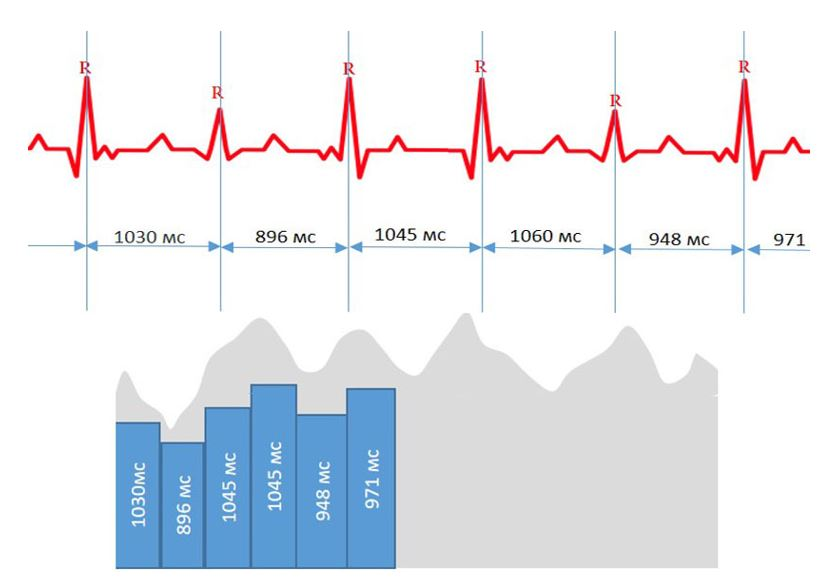
\includegraphics[scale=0.65]{picture-1}}
		\caption{Формирование кардиоинтервалограммы}
		\label{fig:picture-1}
	\end{figure}
	\newpage
	\tableofcontents
\end{document}